\documentclass{article}
\usepackage[utf8]{inputenc}
\title{Lecture 1 Topic}
\author{wbg231 }
\date{December 2022}
\newcommand{\R}{$\mathbb{R}$}
\newcommand{\B}{$\beta$}
\newcommand{\A}{$\alpha$}
\newcommand{\D}{\Delta}

\newcommand{\avector}[2]{(#1_2,\ldots,#1_{#2})}
\newcommand{\makedef}[2]{$\textbf{#1}$:#2 }
\usepackage{tikz,graphicx,hyperref,amsmath,amsfonts,amscd,amssymb,bm,cite,epsfig,epsf,url}

\begin{document}

\maketitle

\section{into to ml}
\begin{itemize}
\item \href{https://nyu-ds1003.github.io/mlcourse/2023/lectures/lec01/01b.intro-machine-learning.pdf}{lecture slides}
\item in machine learning our goal is typically to solve a prediction problem of the format given an input x predict an output y 
\item example problem types are binary classification (predict one of 2 classes), multi class classification (predict one of a number of classes), regression (predict an output that is continuous) 
\subsection{rule based approach}
\item machine learning should be understood in comparison to a rule based approach with the following work flow (consider for example medical diagnosis)
\begin{itemize}
    \item talk to experts (in this case doctors)
    \item understand how the experts come up with a diagnosis.
    \item implement this process as an algorithm or rule based system (eg given a certain set of symptoms output a diagnosis)
    \item try to infer new rules from the rules you are explicitly told 
    \item 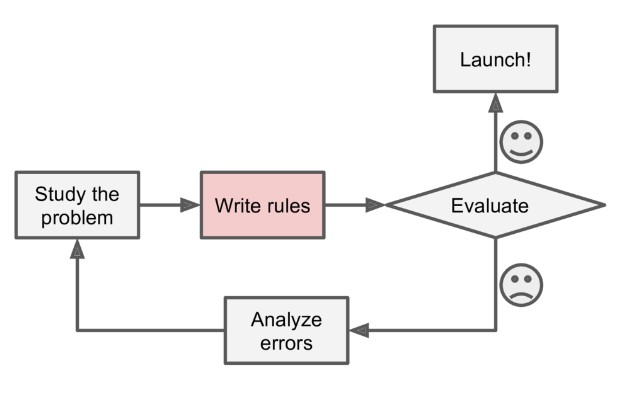
\includegraphics[width=5cm]{lecture_notes/lecture_1/wba.jpg}
\end{itemize}
\item this type of approach has a number of pros 

\begin{itemize}
    \item it leverages preexisting knowledge and expertise
    \item  generally the rules are interpretable 
\item they produce good answers for questions or scenarios included within the knowledge base
\end{itemize}
\item they also have some cons 
\begin{itemize}
    \item they are labor intensive, and the time of experts is expensive
    \item rules don't generalize to novel or not yet seen problems 
    \item rules do not handle uncertainty well
\end{itemize}
\subsection{machine learning approach}
\item in contrast to the rule based approach is the ml approach 
\item instead of explicitly engineering the process that a human expert would use to make a decision we have a machine learn on its own form the inputs and output decision
\item in supervised learning we provide training data with input output pairs (x,y) for which the model to learn from 
\item A machine learning algorithm learns form the training data. takes as input training data and outputs something that we want 
\item the goal of ml is to find the best (to be defined) prediction function automatically based on the training data 
\item our ability too do this well depends on two things 
\begin{itemize}
    \item the availability of large amounts of data for training
    \item how well our model will generalize to unseen cases. 
\end{itemize}
\item here is a diagram of the machine learning approach \item 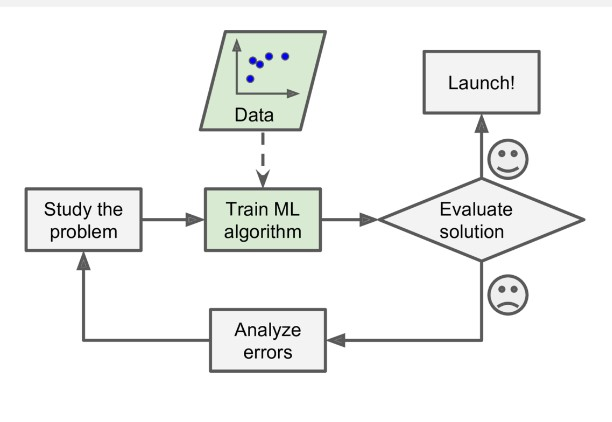
\includegraphics[width=5cm]{lecture_notes/lecture_1/mla.jpg}
\subsection{key concepts}
\item classification (binary, multi class)
\item regression
\item prediction function a function that predicts outputs (y) given input (x)
\item training data a set of inputs x and output y pairs to train the model with
\item supervised learning algorithm takes training data and produces a prediction function 
\item beyond prediction there are concepts such as unsupervised learning, reinforcement learning and representation learning 
\subsection{core questions}
\item the core questions to ask given any machine learning task are 
\begin{itemize}
    \item model: what class of prediction function are we considering
    \item  learning how do we learn the best prediction function in this class from our training data 
    \item inference how do we compute the output of the prediction function for a new input? 
\end{itemize}
\section{statistical learning theory}
\item \href{https://nyu-ds1003.github.io/mlcourse/2023/lectures/lec01/01c.intro-stat-learning-theory.pdf}{lecture notes}
\item in data science problems we generally need to:
\begin{itemize}
    \item make a decision (ie move an email to the spam folder) 
    \item take an action (have a self driving car turn, reject a hypothesis)
    \item produce some output (translate a sentence from English to french, whose face is in an image) 
    \item predict where a storm will be in an hour (output x,y coordinates )
    \item an action is the generic term for what is produced ie the output of our system 
\end{itemize}
\item what we base our decision  off of are either called inputs (in machine learning) or Covariates  (in stats) ex: pictures, a search query, stock price history
\item inputs are often paired with outputs or labels. (does that picture have an animal in it, suggested URLs, should we sell a stock)
\item Decision  theory is all about finding optimal actions under carious definitions of optimally (ie evaluation criteria) ex (is the classification correct, how far off was our prediction) .
\subsection{formalize set up}
\item the problem can be formalized as follows
\begin{itemize}
    \item observe input x
    \item take action a
    \item observe outcome y
    \item evaluate action in relation to the outcome
\end{itemize}
\item there are three spaces to consider. the input space (X), the action space (A), the outcome space(Y)
\item a prediction function (or decision  function) takes an input $x\in X$ and produces an action $a\in A$ \\ $f:X\rightarrow A\\x\rightarrow f(x)$
\item a loss function evaluates the action in the context of the outcome y. $\\ \mathscr{l}:A\times Y\rightarrow\mathbb{R}\\(a,y)\rightarrow \mathscr{l}(a,y)$
\subsection{evaluating a prediction function}
\item our goal is to find the optimal prediction function 
\item the loss function $\ell$ evaluates a single action 
\item but in order to fully evaluate a prediction function as a whole we need to use the statistical learning theory frame work 
\subsection{statistical learning theory framework setup}
\item our first step is to define a space where the prediction function is applicable
\begin{itemize}
    \item assume that there is a data generating process $P_{X\times Y}$ 
    \item all input output pairs (x,y) are generated iid from $P_{X\times Y}$ 
\end{itemize}
\item we want a prediction function that does well on average ie usually has a small loss.
\item to do this we def fine the risk of a prediction function $f:X\rightarrow A$ as $$R(f)=E_{(x,y)~P_{X\times Y}}[\ell (f(x),y)]$$ in words this is the expected loss of f over $P_{X\times Y}$
\item to further clarify the risk is defined as the expected value of our loss function over the input and output space (X,Y) generated by the data generating process $P_{X\times Y}$
\item we can not compute the risk in practice because we don't know the whole data generating process and thus can not compute expectation, but we can estimate it 
\item The Bayes prediction function $f^{*}:X\rightarrow A$ is a function that ac hives the minimal risk among all possible functions $$f^{*}\in argmin_{f}R(f)$$ where the minimum is takes over all functions mapping the input space to the action space. 
\item the risk of the Bayes factor is called the Bayes risk, even the best function will usually have this as it is ineducable 
\item the Bayes prediction function is also called the Target function as it is the best prediction function we could get and thus what we are aiming to learn 
\subsection{example}
\item consider a multi-classification problem with action and output space A=Y=$\{1...k\}$
\item further suppose we take 0-1 loss. 
\begin{equation*}
\ell(a,y) = 1(a\neq y) = \left\{
        \begin{array}{ll}
            1 & \text{ if } a\neq y  \\
            0 & \text{otherwise}
        \end{array}
    \right.
\end{equation*}
\item thus our risk function is $E[f]=E[1f(x)\neq y]=0*P(f(x)=y)+1*P(f(x)\neq y)=P(f(x)\neq y)$ ie just the likely would we misclassify something 
\item so the Bayes prediction function returns the most likely class ie $f^{*}(x)\in argmax_{1\leq c\leq k}P(y=c|x)$ this makes sense as this by definition would result in the minimum possible probability of making a mistake for each input and thus minimizes our risk function
\item despite this we still can not compute risk because we do not know $P_{X\cross Y}$ so we try to estimate it 
\item assume that we have some data of size n $\mathcal{D}_{n}=((x_1,y_1)...(x_n,y_n))$ that is drawn iid from $P_{X\cross Y}$
\item from the law of large numbers we know that if $z_1...z_n$ are drawn at random with expected value $E[z]$ then $lim_{n\rightarrow \infty}\frac{1}{n}\Sigma_{i=1}^{n}z_i=E[z]$ with probability 1. in other words if we draw idd samples  as our sample size gets larger the average of the sample will approach the mean of the distribution it is drawn from 
\item the empirical risk of a prediction function $f:X\rightarrow A$ with respect to the dataset $\mathcal{D}_{n}$ is $$\hat{R}_{n}(f)=\frac{1}{n}\Sigma_{i=1}^{n}\ell(f(x_i),y_i)$$
\item and by the strong law of large numbers $lim_{n\rightarrow \infty}\hat{R}_{n}(f)=R(f)$ 
\item in other words if we take a large enough iid sample from our data generating process our empirical risk will approximate the theoretical risk 
\item given this it is reasonable to try to minimize our empirical risk 
\item a function $\hat{f}$ is an empirical risk minimizer if $$\hat{f}\in argmin_{f}\har{R}_{n}(f)$$  where the min is takes over all functions mapping from x to a.
\item in an ideal world we would want the risk minimizer, but in practice due to finite data the empirical risk minimizer is the best we can hope for 
\subsection{example}
\item suppose we are drawing data from $P_{X\times Y}$ such that x is uniformly distributed on [0,1] and y is always 1. 
\item such a distribution would look like this 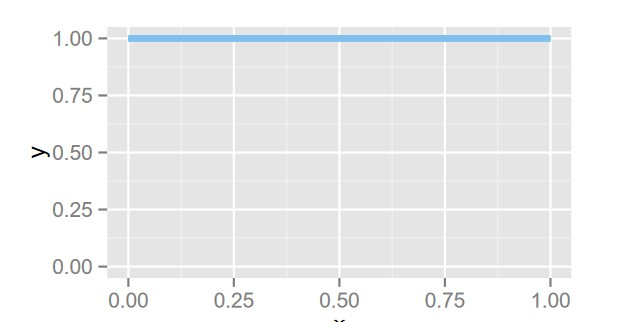
\includegraphics[width=5cm]{lecture_notes/lecture_1/plot_1.jpg}
\item suppose we got data $D_{3}=\{.25,.5,.75\}$ and we deffined our prediction function as \begin{equation*}
f(x) = 1(x\in\{.25,.5,.75\}) = \left\{
        \begin{array}{ll}
            1 & \text{ if } x \in \{.25,.5,.75\}  \\
            0 & \text{otherwise}
        \end{array}
    \right.
\end{equation*}
\item under a 0/1 loss function f would have an empirical risk of 0 and a risk of 1. 
\item so in this case empirical loss minimization let a function f that just memoir zed the data, but clearly this does not generalize well.
\subsection{Constrained ERM}
\item so we want a way to try to smooth things out, that is to extrapolate information we have from out dataset to the unobserved parts of the input space over all 
\item one approach is called constrained  ERM (empirical risk minimization) in which instead of minimizing empirical risk over all prediction functions we constraint our search to a particular subset of the space of functions called a hypothesis space. 
\item A hypothesis space $\mathcal{F}$ is a set of prediction functions $X\rightarrow A$ that we consider during ERM
\item a good hypothesis space should have the following two properties 
\begin{itemize}
    \item include only those functions that have the desired regularity that is properties we want such as smoothness of simplicity
    \item the functions in this space should be easy to work with
\end{itemize}
\item a lot of applies work is about finding a good hypothesis space.
\item an empirical risk minimizer over a hypothesis space $\mathcal{F}$ is a function $\hat{f}_{n}$ such that $$\hat{f}_{n}\in argmin_{f\in \mathcal{F}}\frac{1}{n}\Sigma_{i=1}^{n}\ell(f(x_i),y_i)$$
ie it is the function that minimizes empirical risk within the hypothesis space. 
\item a risk minimizer in $\mathcal{F}$ is a function $f^{*}_{\mathcal{F}}$ such that $$f^{*}_{\mathcal{F}}\in argmin_{f\in \mathcal{F}}E[\ell(f(x),y)]$$
ie a function that minimizer risk in the hypothesis space.
\item the set up for our problem can be visualized like this \item 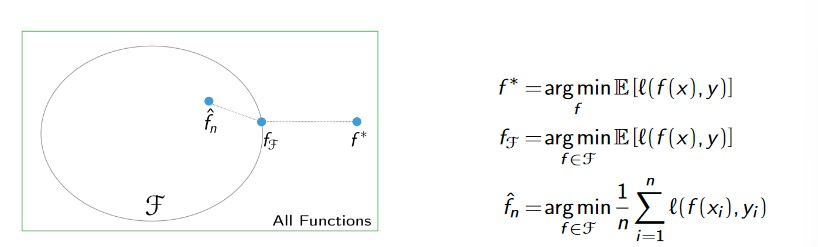
\includegraphics[width=10cm]{lecture_notes/lecture_1/fucntion_sapce.jpg}
\item the approximation error (of $\mathcal{F})=R(f_{\mathcal{f}})-R(f^{*})$ so that is the difference between the lowest risk function overall and the lowest risk function within the hypothesis space, think of this as what we lose by choosing a hypothesis space
\item the estimation error (of $\hat{f}_{n}$ in $\mathcal{F}$)= $R(\hat{f}_{n})-R(f_{\mathcal{F}})$ so that is the distance between the best function find empirically and the best possible function within your space. think of this as what you lose from your data 
\item the excess risk compares the risk of f to the Bayes optimal $f^{*}$ excess risk(f)$=R(f)-R(f^{*})$ thus tells us how much more risk a given function has than the overall optimal function 
\item the excess risk of the ERM $\hat{f}_{n}$ can be decomposed as excess risk$(\hat{f}_{n})=R(\hat{f}_{n})-R(f^{*})=R(\hat{f}_{n})-R(f_{\mathcal{F}})+R(f_{\mathcal{f}})-R(f^{*})$ which is the estimator error plus the approximation error 
\item there is a trade off between estimation and approximation error 
\subsection{approximation error}
\item approximation error $R(f_{\mathcal{F}})-R(f^{*})$ is a property of the class of $\mathcal{F}$, it is the penalty for restricting to $\mathcal{F}$ 
\item a bigger $\mathcal{F}$ means smaller approximation error, 
\item approximation error is a non-random variable
\subsection{estimation error}
\item estimation error $R(\hat{f}_{n})-R(f_{\mathcal{F}}$ is the performance hit for choosing f using finite training data, further it is what we lose for minimizing empirical rather than true risk. 
\item with a smaller $\mathcal{F}$ there are less functions to consider and thus we expect a lower estimation error 
\item under typical conditions with infinite training data estimation error goes to zero
\itme estimation error should be a random quantity. 
\subsection{}{ERM in practice}
\item in practice finding the exact optimum within a space is hard, and does not always work out 
\item so in practice we don't always find $\hat{f}_{n}\in \mathcal{F}$ that is the function with the lowest risk in our hypothesis space instead we find $\Tilde{f}_{n}\in \mathcal{F}$ and hope it is good enough 
\item given $\Tilde{f}_{n}$ is the function our optimization method returns and $\hat{f}_{n}$ is the empirical risk minimize then the optimization error=$R(\Tilde{f}_{n})-R(\hat{f}_{n})$
\item so in practice the excess risk decomposition of the function $\Tilde{f}_{n}$ returned by an optimization algorithm is excess risk($\Tilde{f}_{n})=R(\Tilde{f}_{n})+R(f^{*})=R(\Tilde{f}_{n})-R(\hat{f}_{n})+R(\hat{f}_{n})-R(f_{\mathcal{F}})+R(f_{\mathcal{F}})-R(F^{*})$ which is the sum of optimization error, estimation error and approximation error
\item once again this is not something that we can observe in practice, but instead something to keep in mind during the process. 
\subsection{ERM overview}
\item given a loss function $\ell:a\times y\rightarrow \mathbb{R}$
\item chose a hypothesis space $\mathcal{F}$
\item use an optimization method to find an empirical risk minimizer in the hypothesis space $\hat{f}_{n}\in \mathcal{F}$ such that $\hat{f}_{n}=argmin_{f\in \mathcal{F}}\frac{1}{n}\Sigma_{i=1}^{n}\ell(f(x_i),y_i)$ or at the least fine an $\Tilde{f}_{n}$ close to it 
\item the job of the designer is to chose $\mathcal{F}$ that balances approximation and estimation error 
\item as we get more training data we can pick a larger $\mathcal{F}$
\end{itemize}
\end{document}
